\chapter{Cinétique électrochimique et électroanalyse}\label{ch:b3:electrode-kinetics}

Une goutte de sang sur une bandelette de plastique, cinq secondes, un
nombre~: le lecteur de glycémie que des millions de personnes utilisent
plusieurs fois par jour est une cellule électrochimique, et ce qu'il
mesure n'est pas une tension mais un courant. Une \omterm{def:b3:complex-kinetics:enzyme}{enzyme} oxyde le
glucose, un complexe du fer dissous transporte les électrons jusqu'à une
électrode de carbone, et le courant qui passe est fixé par la vitesse à
laquelle ce complexe diffuse jusqu'à l'électrode, donc par sa
concentration. Ce chapitre explique pourquoi les électrons franchissent
une interface vite ou lentement (l'\omterm{thm:b3:electrode-kinetics:butler-volmer}{équation de Butler--Volmer}), comment
le transport de matière limite le courant, et comment la \omterm{def:b3:electrode-kinetics:cv}{voltampérométrie
cyclique} et les autres méthodes électroanalytiques transforment des
courants en concentrations, en constantes de vitesse et en mécanismes.

\begin{recall}
Le volume de première année a défini le potentiel d'électrode, le
potentiel standard, la relation de Nernst, les électrodes de référence et
les demi-piles. Le volume de deuxième année a introduit les courbes
intensité--potentiel avec leurs courants anodiques et cathodiques,
l'électrode de travail et la contre-électrode, les surtensions, les
systèmes rapides et lents, la couche de diffusion et le courant limite~;
les coefficients d'activité et la force ionique~; les droites
d'étalonnage, la méthode des ajouts dosés et la limite de détection. Le
\Cref{ch:b3:rate-theories} a donné la \omterm{def:b3:rate-theories:tst}{théorie de l'état de transition}.
De la physique~: les lois de Fick de la diffusion, l'équation de Poisson
et les condensateurs.
\end{recall}

\begin{omfigure}
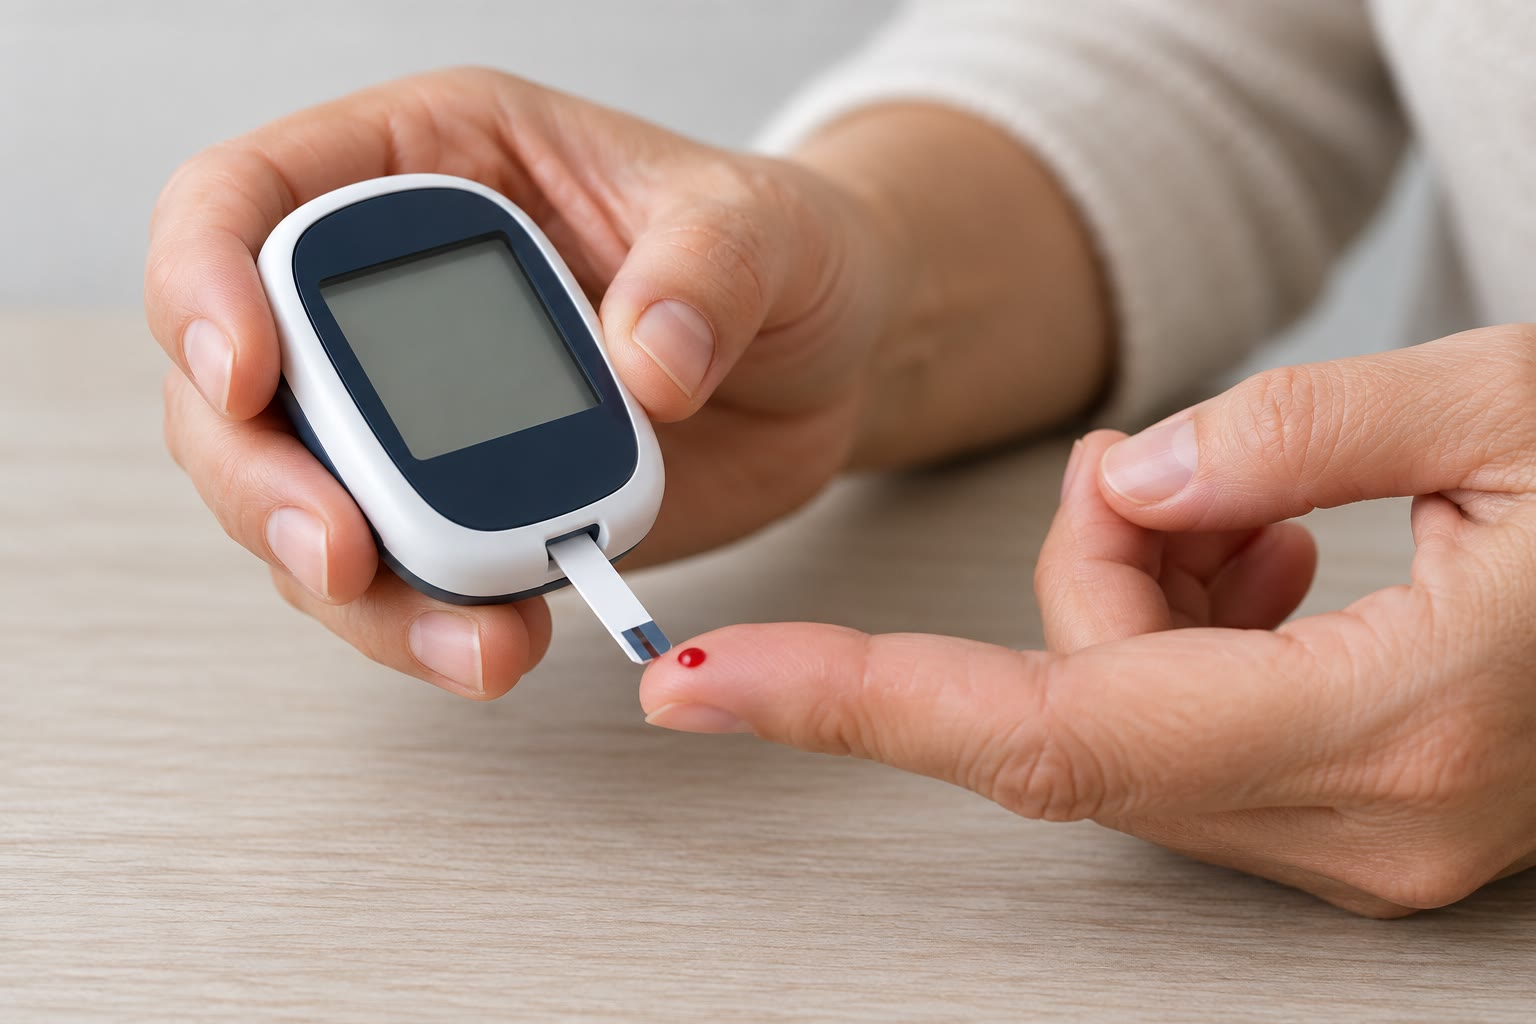
\includegraphics[width=0.6\linewidth]{images/book4/ai/b3-15-glucose-meter.jpg}

{\small Un lecteur de glycémie~: la bandelette porte une minuscule
cellule à trois électrodes, avec une \omterm{def:b3:complex-kinetics:enzyme}{enzyme} et un médiateur rédox~; le
lecteur impose un potentiel et lit un courant.}
\end{omfigure}

\section{L'interface électrode--solution}

Un métal plongé dans une solution d'électrolyte porte une charge de
surface, et la solution lui répond par une charge égale et opposée faite
d'un excès d'ions d'un même signe. Les deux couches de charge forment un
condensateur d'épaisseur moléculaire.

\begin{definition}[Double couche électrique]\label{def:b3:electrode-kinetics:double-layer}
La \emph{double couche électrique}\index{double couche electrique@double couche électrique} est
la distribution des charges à une interface électrode--solution~: la
charge portée par le métal et la charge ionique qui la compense dans la
solution. Sa partie compacte, la
\emph{couche de Helmholtz}\index{couche de Helmholtz}, est la couche
d'ions et de molécules de solvant au contact de la surface~; sa
\emph{couche diffuse}\index{couche diffuse} est la région située au-delà,
où l'agitation thermique répartit les ions en excès sur une distance de
l'ordre de la \emph{longueur de Debye}\index{longueur de Debye} $\kappa^{-1}$. La
\emph{capacité de double couche}\index{capacite de double couche@capacité de double couche} $C_{\mathrm{dl}}$ est la charge
stockée par unité d'aire et par volt de potentiel aux bornes de
l'interface.
\end{definition}

\begin{proposition}[Longueur de Debye]\label{prop:b3:electrode-kinetics:debye-length}
Dans une solution de force ionique $I$ (en \unit{mol.m^{-3}}) et de
permittivité relative
$\varepsilon_r$, un petit potentiel $\varphi_0$ imposé à l'électrode
décroît dans la solution selon
$\varphi = \varphi_0\eu^{-\kappa x}$, avec
\[
  \kappa^{-1} = \sqrt{\frac{\varepsilon_r\varepsilon_0RT}{2F^2I}} .
\]
\end{proposition}

\begin{proof}
L'équation de Poisson (issue de la physique) relie le potentiel à la
densité de charge~:
$\dd^2\varphi/\dd x^2 = -\rho/\varepsilon_r\varepsilon_0$. Chaque ion
suit la \omterm{def:b3:partition-functions:boltzmann}{distribution de Boltzmann} dans le
potentiel~: $c_i = c_i^{\circ}\eu^{-z_iF\varphi/RT}$, donc $\rho = F\sum_iz_ic_i^{\circ}\eu^{-z_iF\varphi/RT}$. Pour $F\varphi \ll RT$,
$\eu^{-z_iF\varphi/RT} \approx 1 - z_iF\varphi/RT$~; les termes d'ordre
zéro se compensent par électroneutralité,
et $\rho \approx -(F^2/RT)\sum_iz_i^2c_i^{\circ}\,\varphi = -(2F^2I/RT)\varphi$. Donc $\dd^2\varphi/\dd x^2 = \kappa^2\varphi$,
dont la solution qui s'annule loin de l'électrode est $\varphi_0\eu^{-\kappa x}$.
\end{proof}

\begin{example}[L'épaisseur de la double couche]\label{ex:b3:electrode-kinetics:debye}
% ledger: eps:H2O.25C, const:eps0, const:F, const:R
Dans l'eau à \qty{298.15}{K} ($\varepsilon_r = 78.4$) avec
\qty{0.10}{mol/L} d'un sel 1:1 ($I = \qty{100}{mol.m^{-3}}$),
$\kappa^{-1} = \sqrt{78.4 \times \num{8.854e-12} \times 2479/(2 \times 96\,485^2 \times 100)} = \qty{0.96}{nm}$~;
à \qty{1.0}{mmol/L}, elle est dix fois plus grande. Un \omterm{def:b3:electrode-kinetics:transport}{électrolyte
support} comprime la \omterm{def:b3:electrode-kinetics:double-layer}{couche diffuse} jusqu'à quelques diamètres
moléculaires.
\end{example}

La \omterm{def:b3:electrode-kinetics:double-layer}{couche diffuse} se comporte comme un condensateur dont les armatures
sont distantes de $\kappa^{-1}$~: sa capacité par unité d'aire à faible
potentiel vaut $\varepsilon_r\varepsilon_0\kappa$ (résultat de
Gouy--Chapman~; sa dépendance en potentiel est admise). En série avec la
couche compacte de Helmholtz, elle donne la $C_{\mathrm{dl}}$ mesurée, de
l'ordre de quelques dizaines de microfarads par centimètre carré (modèle
de Stern). Chaque fois que le potentiel varie, ce condensateur se
charge~: un balayage à $v$ volts par seconde appelle un courant capacitif
$C_{\mathrm{dl}}Av$ qui ne porte aucune chimie et s'ajoute à toute
mesure voltampérométrique.

\begin{omfigure}
\begin{tikzpicture}[font=\small, >=Stealth]
  \fill[black!25] (-1.0,0) rectangle (0,3.2);
  \node[rotate=90] at (-0.5,1.6) {métal};
  \foreach \y in {0.3,0.8,...,2.9}{\node[font=\scriptsize] at (-0.15,\y) {$-$};}
  \foreach \y in {0.35,0.95,1.55,2.15,2.75}{\draw[omDef, fill=omDef!20] (0.3,\y) circle (0.18); \node[font=\scriptsize] at (0.3,\y) {$+$};}
  \draw[black!50, dashed] (0.55,0) -- (0.55,3.2);
  \node[font=\scriptsize, anchor=south, align=center] at (0.45,3.25) {plan de\\ Helmholtz};
  \foreach \x/\y/\s in {1.1/0.6/+, 1.4/2.2/+, 1.9/1.3/+, 2.3/2.7/-, 2.6/0.5/+, 3.1/1.8/+, 3.5/0.9/-, 3.9/2.4/+, 4.4/1.4/-, 4.8/0.4/+, 5.1/2.8/-, 5.4/1.9/+}{
    \draw[black!60, fill=white] (\x,\y) circle (0.15); \node[font=\scriptsize] at (\x,\y) {$\s$};}
  \node[font=\scriptsize, anchor=south] at (3.2,3.25) {couche diffuse};
  \draw[->] (0,-2.1) -- (6.0,-2.1) node[anchor=north east] {$x$};
  \draw[->] (0,-2.1) -- (0,-0.3) node[anchor=east] {$|\varphi|$};
  \draw[omThm, thick] (0,-0.5) -- (0.55,-1.0) plot[domain=0.55:5.8, samples=40] (\x,{-2.1+1.1*exp(-(\x-0.55)/1.2)});
  \draw[black!40, dashed] (0.55,-2.1) -- (0.55,-0.4);
  \node[omThm, anchor=south west] at (1.3,-1.6) {$|\varphi(x)|$};
  \draw[<->, black!60] (0.55,-2.5) -- (1.75,-2.5) node[midway, below, font=\scriptsize] {$\sim\kappa^{-1}$};
\end{tikzpicture}

{\small La \omterm{def:b3:electrode-kinetics:double-layer}{double couche électrique} (modèle de Gouy--Chapman--Stern,
schéma)~: un métal chargé négativement, une couche compacte de cations
au plan de Helmholtz, et une \omterm{def:b3:electrode-kinetics:double-layer}{couche diffuse} où les cations sont plus
nombreux que les anions sur quelques \omterm{def:b3:electrode-kinetics:double-layer}{longueurs de Debye}. En dessous, la
valeur absolue du potentiel (négatif, comme la charge du métal) décroît
linéairement à travers la couche compacte, puis exponentiellement dans
la \omterm{def:b3:electrode-kinetics:double-layer}{couche diffuse}.}
\end{omfigure}

\section{Cinétique du transfert d'électrons}

Considérons la réduction $\mathrm{O} + n\,\mathrm{e}^- \to \mathrm{R}$ sur
une électrode maintenue au potentiel $E$, dont le potentiel d'équilibre
pour la solution au sein de la phase serait $E_{\mathrm{eq}}$. La
surtension vaut $\eta = E - E_{\mathrm{eq}}$.

\begin{definition}[Densité de courant d'échange, coefficient de transfert, constante de vitesse standard]\label{def:b3:electrode-kinetics:exchange}
À l'équilibre, les courants anodique et cathodique sont égaux et
opposés~; leur valeur commune par unité d'aire est la \emph{densité de
courant d'échange}\index{densite de courant d'echange@densité de courant d'échange} $j_0$. Le \emph{coefficient de transfert}
\index{coefficient de transfert} $\alpha$ ($0 < \alpha < 1$) est la
fraction de l'énergie électrique $nF\eta$ qui abaisse la barrière de la
réaction cathodique. La
\emph{constante de vitesse standard}\index{constante de vitesse standard} $k^\circ$ est la
valeur commune des constantes de vitesse cathodique et anodique au
potentiel formel $E^{\circ\prime}$.
\end{definition}

\begin{theorem}[Équation de Butler--Volmer]\label{thm:b3:electrode-kinetics:butler-volmer}
Si les concentrations à la surface sont égales à celles du sein de la
solution (pas de limitation par le transport de matière), la densité de
courant à la surtension $\eta$ vaut, en comptant positivement les
courants anodiques,
\[
  j = j_0\bigl[\eu^{(1 - \alpha)f\eta} - \eu^{-\alpha f\eta}\bigr], \qquad f = \frac{nF}{RT}.
\]
C'est l'\emph{équation de Butler--Volmer}\index{equation de Butler--Volmer@équation de Butler--Volmer}.
\end{theorem}

\begin{proof}
D'après la \omterm{def:b3:rate-theories:tst}{théorie de l'état de transition}, les constantes de vitesse
cathodique et anodique valent
$k_{\mathrm c} = A\eu^{-\Delta G_{\mathrm c}^{\ddagger}/RT}$ et
$k_{\mathrm a} = A\eu^{-\Delta G_{\mathrm a}^{\ddagger}/RT}$. Modifier le
potentiel de l'électrode de $\delta E$
modifie l'enthalpie libre de la réaction $\mathrm{O} + n\,\mathrm{e}^- \to \mathrm{R}$
de $nF\,\delta E$ (les électrons
du métal gagnent $-nF\,\delta E$ d'énergie électrique). Supposons, au
premier ordre, qu'une
fraction $\alpha$ de cette variation porte sur la barrière cathodique et
le reste sur la barrière anodique~: $\Delta G_{\mathrm c}^{\ddagger} \to \Delta G_{\mathrm c}^{\ddagger} + \alpha nF\,\delta E$, $\Delta G_{\mathrm a}^{\ddagger} \to \Delta G_{\mathrm a}^{\ddagger} - (1 - \alpha)nF\,\delta E$.
En mesurant $\delta E$
à partir du potentiel d'équilibre, où les deux courants valent tous deux
$j_0$ en valeur absolue, on obtient $j_{\mathrm c} = j_0\eu^{-\alpha f\eta}$ et $j_{\mathrm a} = j_0\eu^{(1 - \alpha)f\eta}$~;
le courant net est leur différence.
\end{proof}

\begin{corollary}[Résistance de transfert de charge]\label{cor:b3:electrode-kinetics:linear}
Pour $|\eta| \ll RT/nF$, $j = j_0f\eta$~: l'interface se comporte comme
une résistance
$R_{\mathrm{ct}} = RT/(nFi_0)$, avec $i_0 = j_0A$.
\end{corollary}

\begin{proof}
On développe les deux exponentielles au premier ordre~: $j = j_0[(1 - \alpha)f\eta + \alpha f\eta] = j_0f\eta$~;
alors
$\eta/i = 1/(fi_0)$.
\end{proof}

\begin{corollary}[Loi de Tafel]\label{cor:b3:electrode-kinetics:tafel}
Pour $\eta \ll -RT/nF$ (surtension fortement cathodique), le terme
anodique est négligeable et
\[
  \eta = \frac{2.303\,RT}{\alpha nF}\bigl(\log j_0 - \log|j|\bigr):
\]
$\log|j|$ est linéaire en $\eta$, de pente $1/(\text{\qty{118}{mV}})$
par décade à \qty{298}{K} pour $\alpha = 0.5$, $n =
1$. C'est la \emph{loi de Tafel}\index{loi de Tafel}.
\end{corollary}

\begin{proof}
$|j| = j_0\eu^{-\alpha f\eta}$, donc $\ln|j| = \ln j_0 - \alpha f\eta$~; on passe aux logarithmes décimaux.
\end{proof}

\begin{definition}[Résistance de transfert de charge, pente de Tafel]\label{def:b3:electrode-kinetics:charge-transfer}
La \emph{résistance de transfert de charge}\index{resistance de transfert de charge@résistance de transfert de charge} d'une
électrode vaut $R_{\mathrm{ct}} = (\partial\eta/\partial i)_{\eta = 0}$. La \emph{pente de Tafel}\index{pente de Tafel}
est la variation de surtension par décade de courant dans le domaine de
Tafel,
$2.303\,RT/\alpha nF$.
\end{definition}

\begin{omfigure}
\begin{tikzpicture}
\begin{axis}[name=bv, omcv, width=0.47\linewidth, height=5.4cm, xmin=-300, xmax=300, ymin=-40, ymax=40,
  xlabel={$\eta$ / mV}, ylabel={$j/j_0$},
  legend style={font=\scriptsize, draw=none, at={(0.03,0.97)}, anchor=north west}, legend cell align=left]
\addplot[omDef, thick] table[x=eta_mV, y=a3] {figdata/out/bachelor-3-butler-volmer.dat};
\addplot[black, thick] table[x=eta_mV, y=a5] {figdata/out/bachelor-3-butler-volmer.dat};
\addplot[omThm, thick] table[x=eta_mV, y=a7] {figdata/out/bachelor-3-butler-volmer.dat};
\legend{$\alpha = 0.3$, $\alpha = 0.5$, $\alpha = 0.7$}
\draw[black!30] (axis cs:-300,0) -- (axis cs:300,0) (axis cs:0,-40) -- (axis cs:0,40);
\end{axis}
\begin{axis}[at={(bv.east)}, anchor=west, xshift=1.2cm, omcv, width=0.47\linewidth, height=5.4cm,
  xmin=-300, xmax=300, ymin=-1.5, ymax=4, xlabel={$\eta$ / mV}, ylabel={$\log|j/j_0|$},
  unbounded coords=jump]
\addplot[omDef, thick] table[x=eta_mV, y=l3] {figdata/out/bachelor-3-butler-volmer.dat};
\addplot[black, thick] table[x=eta_mV, y=l5] {figdata/out/bachelor-3-butler-volmer.dat};
\addplot[omThm, thick] table[x=eta_mV, y=l7] {figdata/out/bachelor-3-butler-volmer.dat};
\draw[black!40, dashed] (axis cs:-300,2.54) -- (axis cs:0,0);
\draw[black!50] (axis cs:-200,1.85) -- (axis cs:-120,3.3) node[anchor=south, font=\scriptsize, inner sep=1pt] {pente $1/(\qty{118}{mV})$};
\end{axis}
\end{tikzpicture}

{\small L'\omterm{thm:b3:electrode-kinetics:butler-volmer}{équation de Butler--Volmer} ($n = 1$, \qty{298}{K}) pour trois
\omterm{def:b3:electrode-kinetics:exchange}{coefficients de transfert}. À gauche~: le courant est linéaire en $\eta$
près de l'équilibre (la \omterm{def:b3:electrode-kinetics:charge-transfer}{résistance de transfert de charge}) et
exponentiel au-delà~; $\alpha$ le rend dissymétrique.
À droite~: le diagramme de Tafel, dont les branches rectilignes
s'extrapolent à $\log|j/j_0| = 0$
en $\eta = 0$~; le trait en tirets est la droite de Tafel cathodique pour
$\alpha = 0.5$.}
\end{omfigure}

\begin{method}[Une analyse de Tafel]\label{met:b3:electrode-kinetics:tafel-analysis}
\begin{enumerate}
  \item Enregistrer le courant stationnaire en fonction de $\eta$ dans une
        solution agitée, bien au-dessous du courant limite (ou corriger
        du transport de matière).
  \item Tracer $\log|i|$ en fonction de $\eta$~; ajuster la branche
        linéaire au-delà d'environ \qty{100}{mV}.
  \item La pente donne $\alpha$ (ou $1 - \alpha$ sur la branche
        anodique)~; l'ordonnée à l'origine en $\eta = 0$ donne $\log i_0$.
  \item Vérifier~: près de $\eta = 0$, la pente de $i$ en fonction de
        $\eta$ vaut $1/R_{\mathrm{ct}} = nFi_0/RT$.
\end{enumerate}
\end{method}

Les systèmes rapides et lents du volume de deuxième année sont les deux
extrémités de ce tableau~: un système rapide a une grande valeur de
$j_0$, et sa courbe intensité--potentiel monte raide au potentiel
d'équilibre~; un système lent exige une grande surtension avant qu'un
courant passe. La \omterm{def:b3:electrode-kinetics:exchange}{densité de courant d'échange} d'une même réaction varie
de nombreux ordres de grandeur d'un matériau d'électrode à l'autre~: le
dégagement de dihydrogène est rapide sur le platine et extrêmement lent
sur le mercure.

\section{Transport de matière}

\begin{definition}[Modes de transport de matière]\label{def:b3:electrode-kinetics:transport}
Les espèces atteignent une électrode par \emph{migration}\index{migration},
le déplacement des ions dans le champ électrique~; par diffusion, sous
l'effet des gradients de concentration~; et par
\emph{convection}\index{convection}, le mouvement de la solution dans son
ensemble (agitation, rotation, écoulement). Un \emph{électrolyte
support}\index{electrolyte support@électrolyte support} est un sel inerte
ajouté en large excès, qui transporte la quasi-totalité du courant à
travers la solution, de sorte que l'espèce électroactive ne se déplace
que par diffusion et convection.
\end{definition}

\begin{definition}[Chronoampérométrie]\label{def:b3:electrode-kinetics:chronoamperometry}
La \emph{chronoampérométrie}\index{chronoamperometrie@chronoampérométrie} enregistre le courant en
fonction du temps après un saut du potentiel de l'électrode.
\end{definition}

\begin{theorem}[Équation de Cottrell]\label{thm:b3:electrode-kinetics:cottrell}
Après un saut de potentiel en $t = 0$ jusqu'à une valeur où l'espèce
électroactive est consommée dès qu'elle atteint une électrode plane
d'aire $A$, dans une solution au repos contenant un \omterm{def:b3:electrode-kinetics:transport}{électrolyte support},
le courant vaut
\[
  i = nFAc^*\sqrt{\frac{D}{\pi t}},
\]
où $c^*$ est la concentration au sein de la solution et $D$ le
coefficient de diffusion. C'est
l'\emph{équation de Cottrell}\index{equation de Cottrell@équation de Cottrell}.
\end{theorem}

\begin{proof}
La concentration obéit à la seconde loi de Fick $\partial c/\partial t = D\,\partial^2c/\partial x^2$, avec $c(x, 0) = c^*$,
$c(0, t) = 0$ pour $t > 0$ et $c \to c^*$ loin de l'électrode. La fonction $c = c^*\operatorname{erf}(x/2\sqrt{Dt})$, avec
$\operatorname{erf}u = \frac{2}{\sqrt\pi}\int_0^u\eu^{-s^2}\dd s$, satisfait ces conditions~: $\operatorname{erf}0 = 0$, $\operatorname{erf}u \to 1$ quand $u \to \infty$
(pour $t \to 0$ en tout $x > 0$, et loin de l'électrode). Avec $u = x/2\sqrt{Dt}$,
$\partial c/\partial t = c^*\frac{2}{\sqrt\pi}\eu^{-u^2}\partial u/\partial t = -c^*\frac{2}{\sqrt\pi}\eu^{-u^2}\frac{u}{2t}$ et $\partial^2c/\partial x^2 = c^*\frac{2}{\sqrt\pi}(-2u)\eu^{-u^2}\frac{1}{4Dt}$~:
les deux membres de la loi de Fick concordent. Le courant est le flux à
la surface~: $i =
nFAD(\partial c/\partial x)_{x = 0} = nFADc^*\frac{2}{\sqrt\pi}\frac{1}{2\sqrt{Dt}} = nFAc^*\sqrt{D/\pi t}$.
(L'unicité de la solution est
admise.)
\end{proof}

\begin{omfigure}
\begin{tikzpicture}
\begin{axis}[name=pr, width=0.47\linewidth, height=5.2cm, xmin=0, xmax=600, ymin=0, ymax=1.08,
  axis lines=left, xlabel={$x$ / \unit{\micro m}}, ylabel={$c/c^*$},
  tick label style={font=\small}, label style={font=\small},
  legend style={font=\scriptsize, draw=none, at={(0.97,0.03)}, anchor=south east}, legend cell align=left]
\addplot[omDef, thick] table[x=x_um, y=t1] {figdata/out/bachelor-3-cottrell-profiles.dat};
\addplot[black!60, thick] table[x=x_um, y=t2] {figdata/out/bachelor-3-cottrell-profiles.dat};
\addplot[omThm, thick] table[x=x_um, y=t3] {figdata/out/bachelor-3-cottrell-profiles.dat};
\addplot[black, thick, dashed] table[x=x_um, y=t4] {figdata/out/bachelor-3-cottrell-profiles.dat};
\legend{\qty{0.1}{s}, \qty{1}{s}, \qty{4}{s}, \qty{16}{s}}
\end{axis}
\begin{axis}[at={(pr.east)}, anchor=west, xshift=1.3cm, width=0.47\linewidth, height=5.2cm,
  xmin=0, xmax=3.3, ymin=0, ymax=40, axis lines=left, xlabel={$t^{-1/2}$ / \unit{s^{-1/2}}},
  ylabel={$i$ / \unit{\micro A}}, tick label style={font=\small}, label style={font=\small}]
\addplot[omDef, very thick] table[x=tm12, y=i_uA] {figdata/out/bachelor-3-cottrell-current.dat};
\end{axis}
\end{tikzpicture}

{\small \omterm{def:b3:electrode-kinetics:chronoamperometry}{Chronoampérométrie} (modèle~: $D = \qty{1.0e-5}{cm^2.s^{-1}}$, $c^* = \qty{1.0}{mM}$, un disque de
\qty{3}{mm}). À gauche~: la couche d'appauvrissement croît comme
$\sqrt{Dt}$, environ \qty{30}{\micro m} après \qty{0.1}{s}
et \qty{350}{\micro m} après \qty{16}{s}. À droite~: le courant de
Cottrell est proportionnel à
$t^{-1/2}$~; sa pente donne $D$.}
\end{omfigure}

Une solution agitée ou une électrode à disque tournant maintient la
couche de diffusion à une épaisseur constante $\delta$~: le courant
atteint la valeur limite stationnaire $nFADc^*/\delta$
du volume de deuxième année. Pour un disque tournant, $\delta$ décroît
comme l'inverse de la racine carrée de la vitesse de rotation (Levich,
admis), ce qui rend le courant limite
proportionnel à $\sqrt\omega$.

\section{La voltampérométrie cyclique}

\begin{definition}[Voltampérométrie cyclique]\label{def:b3:electrode-kinetics:cv}
La \emph{voltampérométrie cyclique}\index{voltamperometrie cyclique@voltampérométrie cyclique} balaie
linéairement en fonction du temps le potentiel d'une électrode de travail
immobile entre deux bornes, aller et retour, à une vitesse de balayage
$v$, dans une solution au repos, et enregistre le courant. La courbe du
courant en fonction du potentiel est le
\emph{voltampérogramme}\index{voltamperogramme@voltampérogramme}~; chaque
vague présente un \emph{courant de pic}\index{courant de pic} $i_{\mathrm p}$ à son \emph{potentiel de pic}\index{potentiel de pic}
$E_{\mathrm p}$.
\end{definition}

Le pic résulte de deux effets antagonistes. Quand le potentiel dépasse
$E^{\circ\prime}$, la concentration du réactif à la surface diminue (la
relation de Nernst, pour un système rapide) et le courant croît~; mais la
couche appauvrie s'épaissit avec le temps et le flux diminue. Au
balayage retour, le produit, encore proche de l'électrode, est
retransformé.

\begin{definition}[Réversibilité]\label{def:b3:electrode-kinetics:reversibility}
Avec le paramètre de vitesse sans dimension $\Lambda = k^\circ/\sqrt{DnFv/RT}$, qui compare
la vitesse du transfert d'électrons à la vitesse de diffusion imposée par
le balayage, un couple constitue un
\emph{système électrochimiquement réversible}\index{systeme electrochimiquement reversible@système électrochimiquement réversible}
si $\Lambda > 15$ (ses concentrations à la surface obéissent à la
relation de Nernst à tout instant), un \emph{système quasi
réversible}\index{systeme quasi reversible@système quasi réversible} si $15 >
\Lambda > 10^{-2(1 + \alpha)}$, et un \emph{système électrochimiquement
irréversible}\index{systeme electrochimiquement irreversible@système électrochimiquement irréversible}
au-dessous.
\end{definition}

\begin{remark}
Les systèmes rapides et lents du volume de deuxième année correspondent à
cette classification, avec une différence~: la réversibilité dépend ici
de la vitesse de balayage. Le même couple peut être réversible à
\qty{10}{mV/s} et \omterm{def:b3:electrode-kinetics:reversibility}{quasi réversible} à
\qty{10}{V/s}, puisqu'un balayage plus rapide laisse moins de temps au
transfert d'électrons.
\end{remark}

\begin{proposition}[Équation de Randles--Ševčík]\label{prop:b3:electrode-kinetics:randles-sevcik}
Pour une vague réversible sur une électrode plane à \qty{298}{K},
\[
  i_{\mathrm p} = 0.4463\,nFAc^*\sqrt{\frac{nFvD}{RT}},
\]
de sorte que $i_{\mathrm p} \propto \sqrt v$. C'est l'\emph{équation de Randles--Ševčík}\index{equation de Randles--Sevcik@équation de Randles--Ševčík}.
\end{proposition}

\begin{proof}[Démonstration partielle]
Avec les variables $\xi = x\sqrt{nFv/(RTD)}$ et $\theta = nFvt/RT$ (le
balayage de potentiel en unités de
$RT/nF$), la loi de Fick assortie de la condition de Nernst à la surface
ne contient aucun paramètre autre que le potentiel de départ~: le flux
sans dimension est une fonction universelle $\chi(\theta)$. De retour
en unités physiques, $i = nFAc^*\sqrt{nFvD/RT}\,\chi(\theta)$~: tout
courant, y compris celui du pic, varie comme $\sqrt v$. La valeur 0.4463
du maximum de
$\chi$ provient d'une résolution numérique (admise~; la simulation de la
figure la reproduit à 0.1\,\% près).
\end{proof}

\begin{proposition}[Écart entre les pics]\label{prop:b3:electrode-kinetics:delta-ep}
Pour une vague réversible, les pics cathodique et anodique se situent à
environ \qty{28.5}{mV}$/n$
de part et d'autre de $E^{\circ\prime}$ (à \qty{298}{K}, pour un
potentiel d'inversion situé bien au-delà de la vague)~:
$\Delta E_{\mathrm p} \approx 57/n$ mV, indépendamment de la vitesse de
balayage, et $E_{1/2} = (E_{\mathrm{pc}} + E_{\mathrm{pa}})/2 =
E^{\circ\prime}$ quand les deux espèces ont des coefficients de diffusion
égaux.
\end{proposition}

\begin{proof}[Démonstration partielle]
Dans la forme sans dimension de la démonstration précédente, le pic se
produit pour une valeur fixe de $\theta$, c'est-à-dire à un potentiel
fixe par rapport à $E^{\circ\prime}$, quelle que soit $v$~; la symétrie
de la condition de Nernst entre O et R place le pic anodique
symétriquement. La valeur numérique est admise~; la simulation donne
$\pm\qty{28.5}{mV}$, $\Delta E_{\mathrm p} = \qty{57.7}{mV}$.
\end{proof}

\begin{omfigure}
\begin{tikzpicture}
\begin{axis}[name=cv, omcv, width=0.62\linewidth, height=6.4cm, xmin=-320, xmax=320, ymin=-30, ymax=22,
  xlabel={$E - E^{\circ\prime}$ / mV}, ylabel={$i$ / \unit{\micro A}},
  legend style={font=\scriptsize, draw=none, fill=white, fill opacity=0.85, text opacity=1,
  at={(0.01,0.99)}, anchor=north west}, legend cell align=left]
\addplot[black!40, thin] table[x=E_mV, y=i_uA] {figdata/out/bachelor-3-cyclic-voltammetry-v25.dat};
\addplot[omDef!60, thin] table[x=E_mV, y=i_uA] {figdata/out/bachelor-3-cyclic-voltammetry-v50.dat};
\addplot[omDef, thick] table[x=E_mV, y=i_uA] {figdata/out/bachelor-3-cyclic-voltammetry-v100.dat};
\addplot[black, thick] table[x=E_mV, y=i_uA] {figdata/out/bachelor-3-cyclic-voltammetry-v200.dat};
\addplot[omThm, thick, dashed] table[x=E_mV, y=i_uA] {figdata/out/bachelor-3-cyclic-voltammetry-quasi.dat};
\legend{\qty{25}{mV/s}, \qty{50}{mV/s}, \qty{100}{mV/s}, \qty{200}{mV/s}, {quasi-rév., \qty{100}{mV/s}}}
\end{axis}
\begin{axis}[at={(cv.east)}, anchor=west, xshift=1.3cm, width=0.32\linewidth, height=5.0cm,
  xmin=0, xmax=0.5, ymin=0, ymax=30, axis lines=left, xlabel={$\sqrt v$ / \unit{(V/s)^{1/2}}},
  ylabel={$|i_{\mathrm{pc}}|$ / \unit{\micro A}}, tick label style={font=\small}, label style={font=\small}]
\addplot[only marks, mark=*, omDef] table[x=sqrtv, y=ip_uA] {figdata/out/bachelor-3-cyclic-voltammetry-ip.dat};
\addplot[black, domain=0:0.5] {60.06*x};
\end{axis}
\end{tikzpicture}

{\small \omterm{def:b3:electrode-kinetics:cv}{Voltampérogrammes} cycliques simulés par différences finies pour
une réduction
(modèle~: \qty{1.0}{mM}, $D = \qty{1.0e-5}{cm^2.s^{-1}}$, disque de
\qty{3}{mm}, $n = 1$~; courant anodique
positif). Vagues réversibles à quatre vitesses de balayage~: les pics
restent séparés de \qty{57.7}{mV},
centrés sur $E^{\circ\prime}$, et le \omterm{def:b3:electrode-kinetics:cv}{courant de pic} croît comme
$\sqrt v$ (à droite, la droite est l'\omterm{prop:b3:electrode-kinetics:randles-sevcik}{équation de
Randles--Ševčík}). En tirets~: un couple \omterm{def:b3:electrode-kinetics:reversibility}{quasi réversible}
($k^\circ = \qty{2e-3}{cm.s^{-1}}$)
à \qty{100}{mV/s}, aux pics séparés de \qty{162}{mV} et plus bas.}
\end{omfigure}

\begin{method}[Diagnostiquer un voltampérogramme]\label{met:b3:electrode-kinetics:cv-diagnosis}
\begin{enumerate}
  \item Réversible~: $\Delta E_{\mathrm p} \approx 57/n$ mV à toute vitesse de balayage, $|i_{\mathrm{pa}}/i_{\mathrm{pc}}| = 1$, $i_{\mathrm p} \propto \sqrt v$~;
        $E_{1/2}$ donne $E^{\circ\prime}$.
  \item \omterm{def:b3:electrode-kinetics:reversibility}{Quasi réversible}~: $\Delta E_{\mathrm p}$ croît avec la vitesse
        de balayage~; sa valeur donne $k^\circ$.
  \item Irréversible~: pas de pic retour~; le \omterm{def:b3:electrode-kinetics:cv}{potentiel de pic} se déplace
        de $30/\alpha n$ mV par
        décade de vitesse de balayage.
  \item Étape chimique consécutive (mécanisme EC)~: le pic retour est plus
        petit que le pic aller aux balayages lents et se rétablit aux
        balayages rapides, qui prennent la chimie de vitesse.
  \item Espèces adsorbées~: $i_{\mathrm p} \propto v$, et non $\sqrt v$.
\end{enumerate}
\end{method}

Les potentiels dans les solvants non aqueux, où les électrodes de
référence dérivent, sont rapportés à un étalon interne ajouté à la fin
de l'expérience~: le couple ferrocénium/ferrocène, rapide et sage dans la
plupart des solvants organiques.

\begin{method}[Monter une mesure à trois électrodes]\label{met:b3:electrode-kinetics:three-electrode}
\begin{enumerate}
  \item Électrode de travail (carbone vitreux, platine, or) fraîchement
        polie~; contre-électrode (fil de platine) de plus grande aire~;
        électrode de référence (Ag/AgCl, ou fil d'argent avec un étalon
        interne) proche de l'électrode de travail.
  \item Solution de l'analyte (environ 1 mM) avec \qty{0.1}{mol/L}
        d'\omterm{def:b3:electrode-kinetics:transport}{électrolyte support}, dégazée à l'argon (le dioxygène dissous est
        réduit à des potentiels modérément négatifs et ajouterait ses
        propres vagues).
  \item Le potentiostat impose le potentiel entre l'électrode de travail
        et l'électrode de référence et fait passer le courant entre
        l'électrode de travail et la contre-électrode~; aucun courant ne
        traverse la référence.
\end{enumerate}
\end{method}

\begin{omfigure}
\begin{tikzpicture}[font=\small, >=Stealth]
  \begin{scope}[scale=1.5]
    \pic[transform shape] at (0,0) {beaker={0.7}{omWater!60}};
    \pic[transform shape] at (-0.45,0.35) {electrode={black!70}};
    \pic[transform shape] at (0,0.35) {electrode={black!20}};
    \pic[transform shape] at (0.45,0.35) {probe};
  \end{scope}
  \draw[thick] (-1.6,6.0) rectangle (1.6,7.2);
  \node at (0,6.6) {potentiostat};
  \draw[thick, omDef] (-0.675,4.35) |- (-1.0,5.2) -- (-1.0,6.0);
  \draw[thick, black!60] (0,4.35) -- (0,6.0);
  \draw[thick, omThm] (0.675,5.18) |- (1.0,5.5) -- (1.0,6.0);
  \node[omDef, anchor=east, align=right, font=\scriptsize] at (-1.1,5.2) {travail};
  \node[black!70, rotate=90, anchor=north, font=\scriptsize, inner sep=1pt] at (0.06,5.35) {contre};
  \node[omThm, anchor=west, align=left, font=\scriptsize] at (1.1,5.2) {référence};
\end{tikzpicture}

{\small Une cellule à trois électrodes. Le potentiostat contrôle le
potentiel de l'électrode de travail par rapport à l'électrode de
référence, qui ne débite aucun courant, et fait passer le courant par la
contre-électrode.}
\end{omfigure}

\section{Méthodes électroanalytiques}

\begin{definition}[Ampérométrie, biocapteur]\label{def:b3:electrode-kinetics:amperometry}
L'\emph{ampérométrie}\index{amperometrie@ampérométrie} mesure le courant à
potentiel fixe, proportionnel à la concentration de l'espèce qui réagit.
Un
\emph{biocapteur}\index{biocapteur} associe un élément de reconnaissance
biologique (une \omterm{def:b3:complex-kinetics:enzyme}{enzyme}, un anticorps) à un transducteur, ici une
électrode.
\end{definition}

Dans la bandelette, la glucose oxydase oxyde le glucose en
gluconolactone et est régénérée par un médiateur, l'hexacyanoferrate(III),
qui est réduit~; à l'électrode, maintenue à un potentiel où
l'hexacyanoferrate(II) est oxydé, le courant mesure le médiateur formé,
deux par glucose~:
\[
  \ce{C6H12O6 + 2 [Fe(CN)6]^3- -> C6H10O6 + 2 [Fe(CN)6]^4- + 2 H+} .
\]

\begin{definition}[Voltampérométrie de redissolution anodique]\label{def:b3:electrode-kinetics:stripping}
La \emph{voltampérométrie de redissolution anodique}\index{voltamperometrie de redissolution anodique@voltampérométrie de redissolution anodique}
préconcentre un métal en réduisant ses ions sur une électrode pendant
une durée fixe à un potentiel fixe, puis balaie le potentiel dans le
sens anodique et mesure le pic de courant de sa réoxydation, qui est
proportionnel à la concentration dans la solution.
\end{definition}

La préconcentration rend la méthode assez sensible pour des traces de
plomb ou de cadmium dans l'eau potable, au niveau du microgramme par
litre. Comme la sensibilité dépend de la matrice, on l'étalonne dans
l'échantillon lui-même, par ajouts dosés.

\begin{method}[Ajouts dosés en redissolution]\label{met:b3:electrode-kinetics:standard-addition}
\begin{enumerate}
  \item Enregistrer le pic de redissolution de l'échantillon, puis après
        trois ajouts ou plus d'un étalon, chacun élevant la concentration
        d'une quantité connue (petits volumes, pour que la dilution soit
        négligeable ou corrigée).
  \item Ajuster la hauteur de pic en fonction de la concentration ajoutée~:
        une droite.
  \item Son intersection avec l'axe des concentrations vaut l'opposé de
        la concentration de l'échantillon~; propager les écarts-types de
        la droite jusqu'au résultat.
\end{enumerate}
\end{method}

\begin{omfigure}
\begin{tikzpicture}
\begin{axis}[name=sp, omcv, width=0.47\linewidth, height=5.2cm, xmin=-600, xmax=-300, ymin=0, ymax=2.4,
  xlabel={$E$ / mV}, ylabel={$i$ / \unit{\micro A}}]
\addplot[black, thick] table[x=E_mV, y=s0] {figdata/out/bachelor-3-standard-addition-peaks.dat};
\addplot[omDef!50, thick] table[x=E_mV, y=s1] {figdata/out/bachelor-3-standard-addition-peaks.dat};
\addplot[omDef!80, thick] table[x=E_mV, y=s2] {figdata/out/bachelor-3-standard-addition-peaks.dat};
\addplot[omDef, thick] table[x=E_mV, y=s3] {figdata/out/bachelor-3-standard-addition-peaks.dat};
\end{axis}
\begin{axis}[at={(sp.east)}, anchor=west, xshift=1.3cm, width=0.47\linewidth, height=5.2cm,
  xmin=-6, xmax=16, ymin=0, ymax=2.3, axis x line=middle, axis y line=left,
  xlabel={Pb ajouté / \unit{\micro g.L^{-1}}}, ylabel={hauteur de pic / \unit{\micro A}},
  tick label style={font=\small}, label style={font=\small},
  xlabel style={at={(0.5,-0.18)}, anchor=north}]
\addplot[black, thin] table[x=added, y=h] {figdata/out/bachelor-3-standard-addition-line.dat};
\addplot[only marks, mark=*, omDef] table[x=added, y=h] {figdata/out/bachelor-3-standard-addition-points.dat};
\node[font=\scriptsize, anchor=south] at (axis cs:-4.26,0.05) {$-c_0$};
\end{axis}
\end{tikzpicture}

{\small Redissolution anodique du plomb avec trois ajouts dosés (données
de l'\cref{exo:b3:electrode-kinetics:9}). À gauche~: les pics de
redissolution croissent à chaque ajout. À droite~: la droite des moindres
carrés de la hauteur de pic en fonction de la concentration ajoutée
coupe l'axe en l'opposé de la concentration de l'échantillon.}
\end{omfigure}

\begin{definition}[Électrode sélective d'ions, coefficient de sélectivité]\label{def:b3:electrode-kinetics:ise}
Une \emph{électrode sélective d'ions}\index{electrode selective d'ions@électrode sélective d'ions} est une électrode
dont le potentiel, à travers une membrane qui échange préférentiellement
un ion, dépend de l'activité de cet ion. Son \emph{coefficient de
sélectivité}\index{coefficient de selectivite@coefficient de sélectivité} $K_{ij}$ mesure sa réponse à
un ion interférent $j$ relativement à l'ion principal $i$.
\end{definition}

\begin{proposition}[Équation de Nikolsky]\label{prop:b3:electrode-kinetics:nikolsky}
Pour un ion principal $i$ de charge $z_i$ et un ion interférent $j$ de
charge $z_j$,
\[
  E = \text{cste} + \frac{RT}{z_iF}\ln\bigl(a_i + K_{ij}a_j^{z_i/z_j}\bigr) .
\]
C'est l'\emph{équation de Nikolsky}\index{equation de Nikolsky@équation de Nikolsky}.
\end{proposition}

\begin{proof}[Démonstration partielle]
Pour une membrane perméable à $i$ seul, l'égalité des potentiels
électrochimiques de part et d'autre donne un potentiel de type Nernst,
$\frac{RT}{z_iF}\ln a_i$ plus une constante.
Si $j$ peut remplacer $i$ dans la membrane par échange d'ions, avec une
constante d'échange qui définit $K_{ij}$, l'activité de $i$ à la surface
de la membrane est augmentée de
$K_{ij}a_j^{z_i/z_j}$ (la puissance assure l'équilibre des charges dans
l'échange). La démonstration détaillée est admise.
\end{proof}

L'électrode de verre du pH-mètre est la plus ancienne \omterm{def:b3:electrode-kinetics:ise}{électrode sélective
d'ions}~; son erreur alcaline, à pH élevé et à forte concentration en
sodium, est le terme de Nikolsky.

\begin{definition}[Coulométrie]\label{def:b3:electrode-kinetics:coulometry}
La \emph{coulométrie}\index{coulometrie@coulométrie} détermine la quantité
d'une substance à partir de la charge totale passée lors de son
électrolyse complète~: $Q = nFn_{\text{substance}}$ (loi de
Faraday), sans aucun étalonnage.
\end{definition}

\begin{proposition}[Incertitude d'une concentration lue sur une droite d'étalonnage]\label{prop:b3:electrode-kinetics:inverse-prediction}
Pour une droite d'étalonnage $y = a + bx$ ajustée sur $n$ étalons
(écart-type résiduel
$s$, moyenne $\bar y$, $S_{xx} = \sum(x_i - \bar x)^2$), la concentration
d'un échantillon dont la réponse moyenne sur $m$ répétitions est $y_0$
vaut $x_0 = (y_0 - a)/b$, avec l'incertitude-type
\[
  u(x_0) = \frac{s}{b}\sqrt{\frac1m + \frac1n + \frac{(y_0 - \bar y)^2}{b^2S_{xx}}} .
\]
\end{proposition}

\begin{proof}
Écrivons $x_0 = \bar x + (y_0 - \bar y)/b$. Au premier ordre, sa variance vaut $(\operatorname{var}y_0 +
\operatorname{var}\bar y)/b^2 + (y_0 - \bar y)^2\operatorname{var}b/b^4$,
les trois termes n'étant pas corrélés ($\bar y$ et $b$
ne sont pas corrélés, \cref{prop:b3:rate-theories:slope-uncertainty}). Avec $\operatorname{var}y_0 =
s^2/m$, $\operatorname{var}\bar y = s^2/n$ et $\operatorname{var}b = s^2/S_{xx}$,
le résultat s'ensuit.
\end{proof}

L'incertitude est la plus petite au milieu du domaine d'étalonnage et
croît vers ses extrémités~; répéter les lectures de l'échantillon ne
réduit que le premier terme.

\begin{inthelab}[Préparer une électrode de carbone vitreux]
L'électrode est polie sur un feutre avec une suspension d'alumine, selon
un mouvement en huit, rincée, passée brièvement aux ultrasons dans l'eau
et rincée de nouveau. Un \omterm{def:b3:electrode-kinetics:cv}{voltampérogramme} d'un couple connu
(hexacyanoferrate, ferrocène) vérifie que l'écart entre les pics est
proche de la valeur réversible~: un écart plus grand signale une surface
encrassée ou une résistance non compensée. La solution est dégazée à
l'argon pendant dix minutes et maintenue sous atmosphère d'argon pendant
les balayages.
\end{inthelab}

\begin{safety}{\ghs[0.62cm]{GHS03}\ghs[0.62cm]{GHS05}\ghs[0.62cm]{GHS07}\ghs[0.62cm]{GHS08}\ghs[0.62cm]{GHS09}}
% ledger: ghs4:PbNO32, ghs4:K3FeCN6
Nitrate de plomb, utilisé pour les étalons de plomb~: comburant, peut
nuire à la fertilité et au fœtus, cancérogène suspecté, très toxique
pour les organismes aquatiques~; les solutions étalons sont achetées
toutes prêtes et manipulées avec des gants, et tous les déchets de plomb
sont collectés. Hexacyanoferrate(III) de potassium~: nocif et suspecté
de nuire à la fertilité~; jamais fortement acidifié ni chauffé (il
pourrait libérer du cyanure d'hydrogène). Les électrodes de mercure,
autrefois courantes en analyse par redissolution, ont été remplacées par
des électrodes à film de bismuth et de carbone.
\end{safety}

\begin{history}[Le polarographe de Heyrovský, 1922]
Jaroslav Heyrovský mesura en 1922 le courant traversant une électrode de
mercure qui s'égouttait d'un fin capillaire, renouvelant sa surface
toutes les quelques secondes, en fonction du potentiel appliqué. Chaque
espèce réductible donnait une vague dont la position l'identifiait et
dont la hauteur mesurait sa concentration~; avec Masuzo Shikata, il
construisit en 1924 le polarographe, qui enregistrait les courbes
automatiquement sur papier photographique. La polarographie fut la
première méthode instrumentale d'analyse chimique d'usage courant, et
valut à Heyrovský le prix Nobel de chimie 1959.
\end{history}

\section{Exercices}

\begin{exercise}[$\star$]\label{exo:b3:electrode-kinetics:1}
Un diagramme de Tafel d'une réduction ($n = 1$, \qty{298}{K}) a une pente
cathodique de $-\qty{118}{mV}$
par décade et s'extrapole en $\eta = 0$ à $|j| = \qty{2.0e-6}{A.cm^{-2}}$
(données de l'exercice). Donner $\alpha$ et $j_0$.
\end{exercise}

\begin{exercise}[$\star$]\label{exo:b3:electrode-kinetics:2}
Une électrode de \qty{0.20}{cm^2} a $j_0 = \qty{1.0e-3}{A.cm^{-2}}$ pour
un couple à un électron. Calculer sa \omterm{def:b3:electrode-kinetics:charge-transfer}{résistance de transfert de charge} à
\qty{298}{K}.
\end{exercise}

\begin{exercise}[$\star$]\label{exo:b3:electrode-kinetics:3}
% ledger: eps:H2O.25C
Calculer la \omterm{def:b3:electrode-kinetics:double-layer}{longueur de Debye} dans l'eau à \qty{298.15}{K} pour
\qty{1.0}{mmol/L} et pour \qty{0.10}{mol/L}
de \ce{MgSO4}.
\end{exercise}

\begin{exercise}[$\star$]\label{exo:b3:electrode-kinetics:4}
Un \omterm{def:b3:electrode-kinetics:cv}{voltampérogramme} cyclique à \qty{100}{mV/s} sur une électrode de
\qty{0.0707}{cm^2} avec $C_{\mathrm{dl}} =
\qty{20}{\micro F.cm^{-2}}$~: calculer le courant capacitif, et le
comparer au pic faradique de
\qty{19}{\micro A} de la figure. Que se passe-t-il à \qty{10}{V/s}~?
\end{exercise}

\begin{exercise}[$\star\star$]\label{exo:b3:electrode-kinetics:5}
Après un saut de potentiel, $i\sqrt t = \qty{12.2}{\micro A.s^{1/2}}$
pour la réduction à un électron d'une solution à
\qty{1.00}{mM} sur une électrode de \qty{0.0707}{cm^2}. Calculer $D$.
\end{exercise}

\begin{exercise}[$\star\star$]\label{exo:b3:electrode-kinetics:6}
Calculer le \omterm{def:b3:electrode-kinetics:cv}{courant de pic} de Randles--Ševčík pour $n = 1$,
$A = \qty{0.0707}{cm^2}$, $c^* = \qty{2.0}{mM}$,
$D = \qty{7.0e-6}{cm^2.s^{-1}}$ à \qty{50}{mV/s} et à \qty{500}{mV/s}.
\end{exercise}

\begin{exercise}[$\star\star$]\label{exo:b3:electrode-kinetics:7}
Trois couples donnent, à 50 et à \qty{500}{mV/s}~: (a) $\Delta E_{\mathrm p} = 58$ et 59 mV, $|i_{\mathrm{pa}}/i_{\mathrm{pc}}| = 1.0$~;
(b) $\Delta E_{\mathrm p} = 75$ et 140 mV, $|i_{\mathrm{pa}}/i_{\mathrm{pc}}| = 1.0$~; (c) $\Delta E_{\mathrm p}$
non défini à \qty{50}{mV/s} (pas de
pic retour), un pic retour avec $|i_{\mathrm{pa}}/i_{\mathrm{pc}}| = 0.8$ à \qty{500}{mV/s}. Diagnostiquer chacun.
\end{exercise}

\begin{exercise}[$\star\star$]\label{exo:b3:electrode-kinetics:8}
Une électrode sélective du potassium a $K_{\ce{K+},\ce{Na+}} = \num{2e-4}$.
Dans un échantillon où $a(\ce{K+}) =
\qty{4.0e-3}{}$ et $a(\ce{Na+}) = 0.14$, quelle est l'erreur relative
sur l'activité du potassium si l'on ignore le sodium~?
\end{exercise}

\begin{exercise}[$\star\star$]\label{exo:b3:electrode-kinetics:9}
Les pics de redissolution d'un échantillon d'eau additionné de 0, 5, 10 et
\qty{15}{\micro g.L^{-1}} de plomb valent 0.468, 1.003, 1.571 et
\qty{2.101}{\micro A} (données de l'exercice). Calculer la concentration
en plomb de la solution mesurée, avec son incertitude-type.
\end{exercise}

\begin{exercise}[$\star\star\star$]\label{exo:b3:electrode-kinetics:10}
Un coulomètre à cuivre fait passer un courant constant de \qty{50.0}{mA}
pendant \qty{30.0}{min} et dépose du cuivre
à partir de \ce{Cu^{2+}}. Calculer la masse déposée~; pourquoi la
\omterm{def:b3:electrode-kinetics:coulometry}{coulométrie} n'exige-t-elle aucun étalonnage~?
\end{exercise}

\begin{exercise}[$\star\star\star$]\label{exo:b3:electrode-kinetics:11}
Pour un couple avec $k^\circ = \qty{1.0e-2}{cm.s^{-1}}$ et $D = \qty{1.0e-5}{cm^2.s^{-1}}$, calculer $\Lambda$ à \qty{0.1}{V/s}
et à \qty{10}{V/s} ($n = 1$, \qty{298}{K}) et classer la vague à chaque
vitesse de balayage.
\end{exercise}

\begin{exercise}[$\star\star\star$]\label{exo:b3:electrode-kinetics:12}
Une droite d'étalonnage établie avec $n = 7$ étalons a $b = \qty{0.919}{\micro A.mM^{-1}}$, $s = \qty{0.077}{\micro A}$,
$\bar y = \qty{8.89}{\micro A}$ et $S_{xx} = \qty{241}{mM^2}$. Calculer
l'incertitude d'une concentration lue à partir d'une lecture en
$y_0 = \bar y$ et en $y_0 = \qty{18.0}{\micro A}$, et à partir de trois
lectures en $\bar y$.
\end{exercise}

\section{Problème~: la bandelette de glycémie}

\begin{problem}[{Problème du week-end --- la bandelette de glycémie~:
l'enzyme et son médiateur, la chronoampérométrie et le coefficient de
diffusion, la droite d'étalonnage et un échantillon de sang avec son
incertitude, et l'interférence de l'ascorbate}]
\label{pb:b3:electrode-kinetics:1}
% ledger: const:F
Une bandelette porte de la glucose oxydase, de l'hexacyanoferrate(III) de
potassium et une électrode de travail en carbone de \qty{0.0300}{cm^2}.
Données du problème~: (a) une bandelette remplie
d'hexacyanoferrate(II) à \qty{10.0}{mM} et portée par un saut à un
potentiel oxydant
donne les courants 42.0, 29.3, 24.1, 20.8 et \qty{18.7}{\micro A} à 1,
2, 3, 4 et \qty{5}{s}~;
(b) des étalons de glucose à 2.0, 4.0, 6.0, 8.0, 10.0, 15.0 et
\qty{20.0}{mM} donnent, à
\qty{5.0}{s}, 2.16, 4.08, 5.83, 7.78, 9.45, 14.23 et \qty{18.69}{\micro A}~;
(c) un échantillon de sang donne
\qty{7.10}{\micro A}.

\medskip\noindent\textbf{Partie I --- La chimie.}
\begin{enumerate}
  \item Écrire les demi-équations du glucose (oxydé en gluconolactone,
        \ce{C6H10O6}) et du médiateur, ainsi que l'équation bilan
        équilibrée.
  \item Combien d'électrons atteignent l'électrode par molécule de
        glucose~?
  \item Pourquoi utilise-t-on un médiateur plutôt que le dioxygène, le
        partenaire naturel de l'\omterm{def:b3:complex-kinetics:enzyme}{enzyme}~?
  \item Pourquoi maintient-on l'électrode à un potentiel où
        l'hexacyanoferrate(II) est oxydé, bien au-delà de son potentiel
        formel~?
  \item Pourquoi faut-il faire la lecture à un instant fixe après le
        dépôt de la goutte~?
\end{enumerate}

\medskip\noindent\textbf{Partie II --- La \omterm{def:b3:electrode-kinetics:chronoamperometry}{chronoampérométrie}.}
\begin{enumerate}[resume]
  \item Quelle loi les courants de (a) doivent-ils suivre~? La vérifier
        sur les données.
  \item Ajuster $i$ en fonction de $t^{-1/2}$ par une droite passant par
        l'origine~: la pente vaut \qty{41.8}{\micro A.s^{1/2}}. En déduire
        $D$ de l'hexacyanoferrate(II).
  \item Calculer l'épaisseur $\sqrt{\pi Dt}$ de la couche
        d'appauvrissement après \qty{5}{s}. Le modèle plan est-il
        raisonnable pour une bandelette dont la couche de solution a une
        épaisseur d'environ
        \qty{100}{\micro m}~?
  \item Quel serait le courant à \qty{5}{s} avec \qty{5.0}{mM} au lieu de
        \qty{10.0}{mM}~?
\end{enumerate}

\medskip\noindent\textbf{Partie III --- L'étalonnage.}
\begin{enumerate}[resume]
  \item La droite des moindres carrés de (b) a $a = \qty{0.356}{\micro A}$ ($s_a = 0.054$), $b =
        \qty{0.9189}{\micro A.mM^{-1}}$ ($s_b = 0.0049$), $s = \qty{0.077}{\micro A}$.
        Que représente $a$~?
  \item La réponse est-elle linéaire sur tout le domaine~? Qu'est-ce qui
        la limiterait aux fortes concentrations de glucose~?
  \item Calculer la concentration en glucose de l'échantillon de sang.
  \item Avec $\bar y = \qty{8.89}{\micro A}$ et $S_{xx} = \qty{241}{mM^2}$,
        calculer son incertitude-type.
  \item Quel terme de l'incertitude domine, et comment pourrait-on le
        réduire~?
  \item Estimer la limite de détection par $3s/b$.
  \item Exprimer le résultat en milligrammes par décilitre (masse molaire
        du glucose
        \qty{180.16}{g/mol}).
\end{enumerate}

\medskip\noindent\textbf{Partie IV --- Les interférents.}
\begin{enumerate}[resume]
  \item L'ascorbate (la vitamine C) est oxydé directement à l'électrode.
        Quel est son effet sur la lecture~?
  \item Comment un \omterm{def:b3:electrode-kinetics:cv}{voltampérogramme} cyclique de la bandelette le
        révélerait-il~?
  \item Pourquoi un potentiel de travail plus bas, rendu possible par un
        meilleur médiateur, réduit-il de telles interférences~?
  \item Une électrode témoin sans \omterm{def:b3:complex-kinetics:enzyme}{enzyme}, lue au même instant, donne
        \qty{0.25}{\micro A} de plus que l'ordonnée à l'origine de
        l'étalonnage avec un échantillon donné. Comment l'utilise-t-on~?
  \item Comment la température de la bandelette influe-t-elle sur le
        courant, par l'intermédiaire de $D$~?
  \item Pourquoi prépare-t-on les étalons dans une matrice semblable au
        sang~?
  \item Pourquoi l'incertitude du lecteur est-elle en pratique plus
        grande que celle calculée dans la partie III~?
  \item Énoncer le résultat~: la concentration en glucose de
        l'échantillon, avec son incertitude-type.
\end{enumerate}
\end{problem}
